%%%%%%%%%%%%%%%%%%%%%%%%%%%%%%%%%%%%%%%%%%%%%%%%%%%%%%%%%%%%%%%%%%%%%%%%%%
\section{E field using cathode-anode piercing tracks}\label{sec:CAMethod}
%%%%%%%%%%%%%%%%%%%%%%%%%%%%%%%%%%%%%%%%%%%%%%%%%%%%%%%%%%%%%%%%%%%%%%%%%%
\begin{figure}[b]
\centering
\begin{minipage}{0.45\textwidth}
\centering
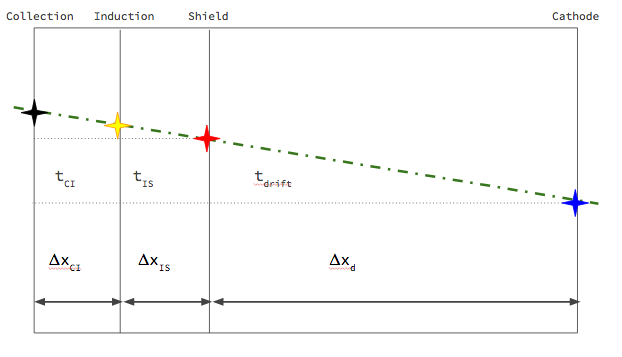
\includegraphics[width=3in]{images/TPCCrossSectionView.png}
\caption{Pictorial representation of the YX view of the TPC. The distance within the anode planes and between the shield plane and the cathode is purposely out of proportion to illustrate the time difference between hits on collection and induciton. A ACP track is shown as an example.}
\label{fig:Scheme}
\end{minipage}\hfill
\begin{minipage}{0.45\textwidth}
\centering
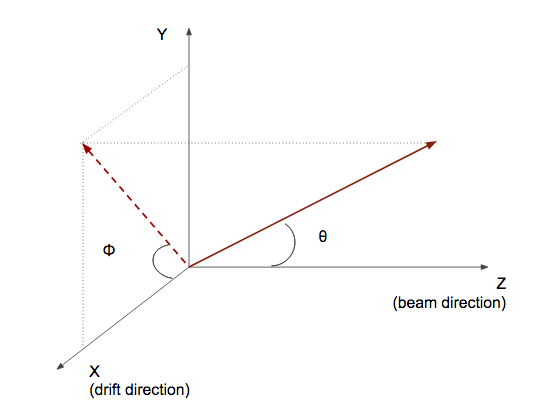
\includegraphics[width=3in]{images/AngleDef.png}
\caption{Angle definition in the context of LArIAT coordinates system.}
\label{fig:AngleDef}
\end{minipage}
\end{figure}

In this section, we utilize a method to measure the drift time (and consequently drift velocity and electric field) using TPC cathode to anode piercing tracks.
The basic idea is simple:
\begin{itemize}
\item[0.] Select cosmic ray events with only 1 reconstructed track 
\item[1.] Select tracks that cross both anode and cathode
\item[2.] Identify the first and last hit of the track
\item[3.] Measure the time difference between these two hits ($\Delta t$),
\item[4.] Derive the drift time from this time difference using the fact that one time tick in TDC is 0.128 $\mu$s.
\end{itemize}
This method works under the assumptions: 
\begin{itemize}
\item [A1.] the selected tracks are minimum ionizing tracks
\item [A2.] the time it takes for a particle to cross the chamber ($\sim$ns) is small compared to the charge drift time ($\sim$ hundreds of $\mu$s).
\end{itemize}

We select events with only one reconstructed track to assure the track considered in the analysis is associated with the trigger and thus we know when the readout began. We utilize anode to cathode piercing tracks (ACP tracks) because their hits span the full drift length of the TPC, see figure \ref{fig:Scheme} and thus allows us define where the first and last hit of the tracks are located in space regardless of our assumption of the electric field. The definition of the last hit is easy: it is the hit closest to the cathode. The definition of the first hit is a bit more complicated. A track that crosses the anode planes will deposit charge in the small drift volumes (S-I and I-C). The drift time in S-I and I-C region was already calculated in Table \ref{tab:Efields}. This is to say that the position of the first hit matters when calculating the drift time at the microsecond precision.
Single hits on the collection plan will not form a 3D object. This means that we can safely exclude that the reconstruction of ACP tracks starts at the cathode plane (black point in figure \ref{fig:Scheme}). %Understanding if the first hit of a track in on the induction or on the shield plan is more complicated. For now, we'll take an uncertainty hit of 2.3 $\mu$s.


One of the main features of this method is that it doesn't rely on the measurement of the trigger time. Since $\Delta t$ is the time difference between the first and last hit of a track and we assume the charge started drifting at the same time for both hits (assumption A2), the measurement of the absolute beginning of drift time $t_0$ is unnecessary. 

%%%%%%%%%%%%%%%%%%%%%%%%%%%%%%%%%%%%%%%%%%%%%%%%%%%%%%%%%%%%%%%%%
\subsection{Andode-Cathode Piercing Tracks Sample Selection}\label{sec:SampleSelectionCA}

The data samples used for this measurement span RunI and RunII. The data are divided into three independent subsamples: RunI positive polarity data, RunII positive polarity data and RunII negative polarity data. Since we're interested in cosmic data, this polarity of the magnet setting is arbitrary and only used to clearly define the data taking period. More details are shown in Table \ref{tab:samples}, while the samweb definitions are defined at the end of \href{https://redmine.fnal.gov/redmine/projects/lardbt/wiki/Recommended_SAM_Datasets}{this wiki page}.

\begin{center}
\begin{table}[htb]
  \begin{center}
    %\resizebox{0.45\textwidth}{!}{%
    \begin{tabular}{c|c|c|c}
      \multicolumn{4}{c}{\textbf{Summary of Samples}} \\
      \hline \hline
       Run Period & LArIATsoft Version & Data Polarity  & SamWeb definition\\
       \hline
       Run-I & \verb!v06_34_01! & Positive &  \verb!Lovely1_Pos_RunI_elenag_v04!\\
       \hline
       Run-II & \verb!v06_34_01! & Positive  & \verb!Lovely1_Pos_RunII_elenag_v04! \\
       \hline
       Run-II & \verb!v06_34_01! & Negative  & \verb!Lovely1_Neg_RunII_elenag_v04! \\
       \hline
       \end{tabular}%}
    \caption{Summary of the data samples used for the Anode-Cathode Piercing tracks study. }
    \label{tab:samples}
    \end{center}
\end{table}
\end{center}

For each sample, the same event selection is used, outlined here:
\begin{itemize}
\item \textbf{Time Stamp Filter}

A filter is used to select events which occured outside the beam window. This is because the beam is mainly focused in the Z direction, so ACP tracks are unlikely to occur during the beam spill. Cosmics events typically occur 5.5 seconds past the beam spill, and therefore the events are filtered using the following LArIATsoft settings

\begin{verbatim}
tfilt:      @local::lariat_timestampfilter

# ====================================================================
# Specify range of events to select.  For Run I/II:
#   - pedestal events:  ~ 0.  - 1.2 sec
#   - beam events:      ~ 1.2 - 5.5 sec
#   - cosmic events:    ~ > 5.5 sec
#   (default selects ALL events)
physics.filters.tfilt.T1:                       5.5
physics.filters.tfilt.T2:                       100.
physics.filters.tfilt.RequireRawDigits:         true

\end{verbatim}


\item \textbf{LArTPC Reconstruction}

Events are then reconstructed inside the TPC. Since we only want ACP tracks, we select tracks that satisfy the following requirements

\begin{itemize}
\item vertical position (Y) of first and last hits within $\pm$ 18 cm from TPC center (avoid Top-Bottom tracks) 
\item horizonatl position (Z) of first and last hits within 2 and 86 cm from TPC front face (avoid throughoing tracks) 
\item longest track with track lenght greater than 48 cm
\item angle from the drift direction (phi in figure \ref{fig:AngleDef}) smaller than 50 deg 
\item angle from the beam direction (theta in figure \ref{fig:AngleDef}) grater than 50 deg
\end{itemize}




\end{itemize}

Tracks passing all these selection requirements are used for the $\Delta t$ calculation.

%%%%%%%%%%%%%%%%%%%%%%%%%%%%%%%%%%%%%%%%%%%%%%%%%%%%%%%%%%%
\subsection{Hit timing information}\label{sec:HitTime}
%%%%%%%%%%%%%%%%%%%%%%%%%%%%%%%%%%%%%%%%%%%%%%%%%%%%%%%%%%%
For each track passing our selection, we loop through the associated hits in order to retrieve the timing information. Hits on the collection plane and induction plane are treated separately. Three types of timing information are provided per each hit: tStart, tPeak and tEnd. The quantities tStart and tEnd are used to identify a region of interest on the signal wave form in each wire. This ROI is represent the time boundary where a fit for the signal peak is performed. The variable tPeak stores the fitted value for the time of the hit. For this analysis, we use \verb!Gaushitfinder! and the variable tPeak as a measure of the hit time.


Figure \ref{fig:RunIPosACP} represents the difference in time between the last and first hit of the selected ACP tracks for Run-I Positive Polarity sample. The red histogram represents $\Delta$t calculated with hits on induction plan, while the blue histogram histogram represents $\Delta$t calculated with hits on the collection plan. Figures \ref{fig:RunIIPosACP} and \ref{fig:RunIINegACP} are analogous and represent Run-II Positive and Negative polarity respectively.



\begin{figure}[]
\centering
\begin{minipage}{0.45\textwidth}
\centering
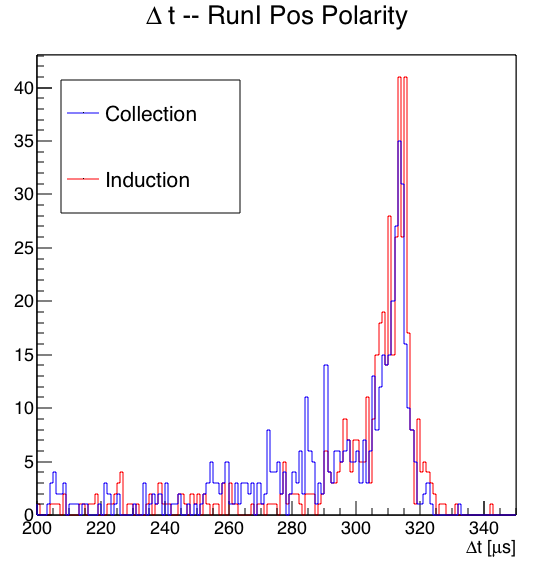
\includegraphics[width=3in]{images/ACPRunIPos.png}
\caption{$\Delta$t for Run I positive polarity data ACP selected tracks. The blue line represents hits on the collection plan, red induction.}
\label{fig:RunIPosACP}
\end{minipage}\hfill
\begin{minipage}{0.45\textwidth}
\centering
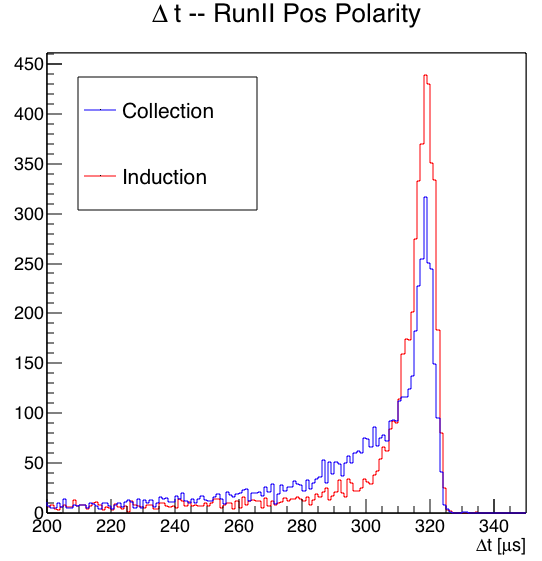
\includegraphics[width=3in]{images/ACPRunIIPos.png}
\caption{$\Delta$t for Run II positive polarity data ACP selected tracks.  The blue line represents hits on the collection plan, red induction.}
\label{fig:RunIIPosACP}
\end{minipage}\hfill
\begin{minipage}{0.45\textwidth}
\centering
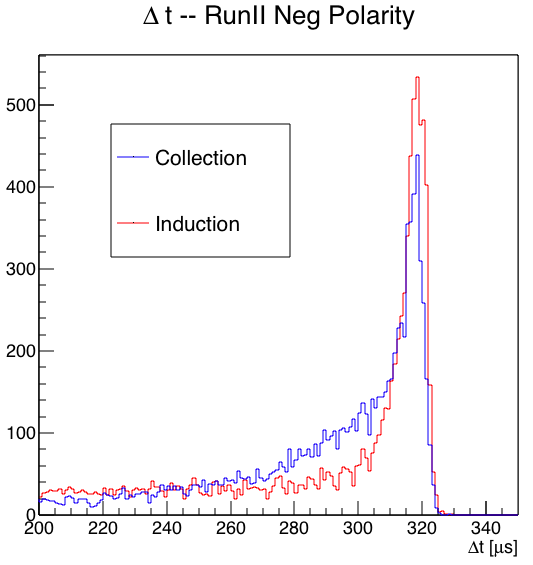
\includegraphics[width=3in]{images/ACPRunIINeg.png}
\caption{$\Delta$t for Run II negative polarity data ACP selected tracks.  The blue line represents hits on the collection plan, red induction.}
\label{fig:RunIINegACP}
\end{minipage}
\end{figure}

\newpage
\clearpage

We fit with a Gaussian to the peak of the $\Delta t$ distributions to extract the mean drift time and the uncertainty associated with it. The fit for Run-I positive polarity is given for the collection plane in Figure \ref{fig:Run1PosCollFit} and for the induction plane in Figure \ref{fig:Run1PosIndFit}. Similar plots for Run-II positive and negative polarity are given in Figures \ref{fig:Run2PosColFit} - \ref{fig:Run2NegIndFit}.

   
\begin{figure}[h!]
\centering
\begin{minipage}{0.40\textwidth}
\centering
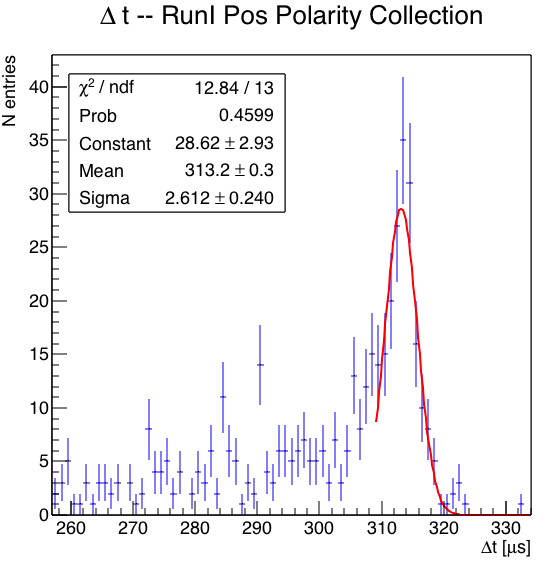
\includegraphics[width=3in]{images/RunIPosCol.png}
\caption{Collection plane $\Delta$t fit  for Run I positive polarity ACP data selected tracks. }
\label{fig:Run1PosCollFit}
\end{minipage}\hfill
\begin{minipage}{0.40\textwidth}
\centering
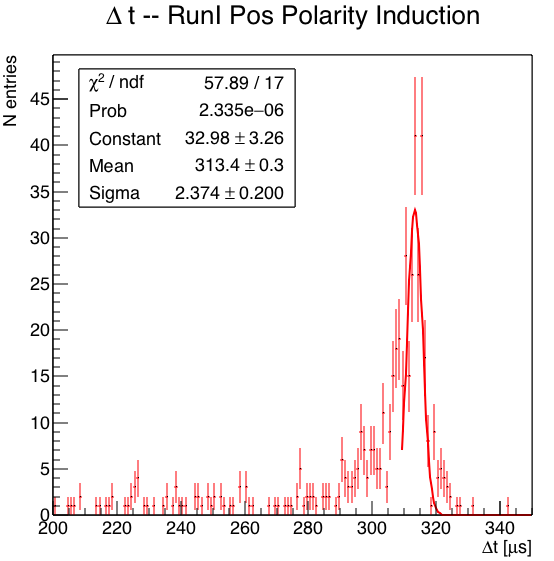
\includegraphics[width=3in]{images/RunIPosInd.png}
\caption{Induction plane $\Delta$t fit  for Run I positive polarity ACP data  selected tracks.}
\label{fig:Run1PosIndFit}
\end{minipage}
\begin{minipage}{0.40\textwidth}
\centering
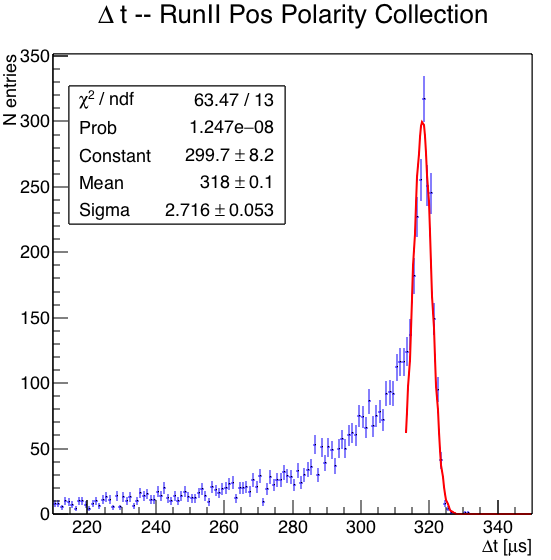
\includegraphics[width=3in]{images/RunIIPosCol.png}
\caption{Collection plane $\Delta$t fit for Run II positive polarity ACP data  selected tracks.}
\label{fig:Run2PosColFit}
\end{minipage}\hfill
\begin{minipage}{0.40\textwidth}
\centering
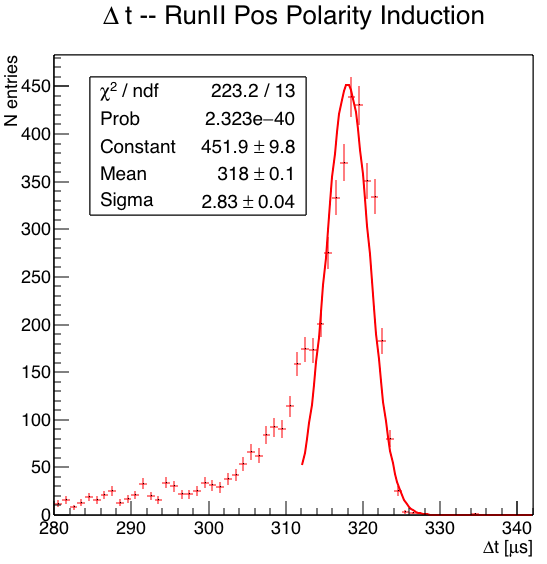
\includegraphics[width=3in]{images/RunIIPosInd.png}
\caption{Induction plane $\Delta$t fit for Run II positive polarity ACP data  selected tracks.}
\label{fig:Run2PosIndFit}
\end{minipage}
\begin{minipage}{0.40\textwidth}
\centering
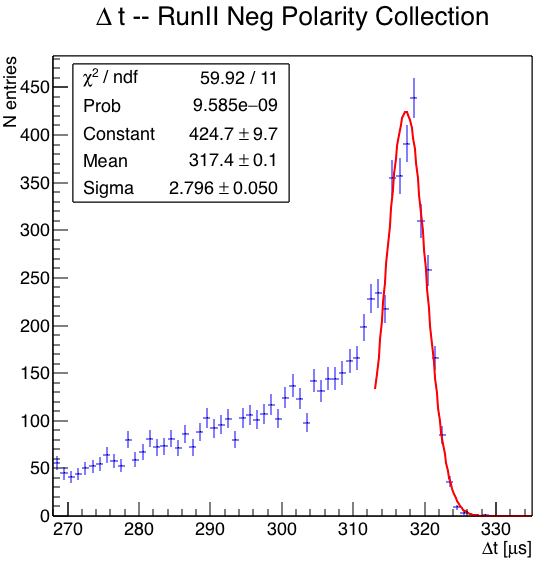
\includegraphics[width=3in]{images/RunIINegCol.png}
\caption{Collection plane $\Delta$t fit for Run II negative polarity ACP data  selected tracks.}
\label{fig:Run2NegColFit}
\end{minipage}\hfill
\begin{minipage}{0.40\textwidth}
\centering
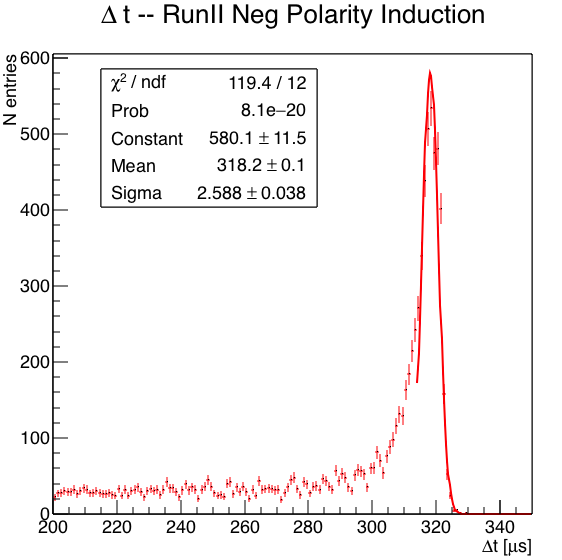
\includegraphics[width=3in]{images/RunIINegInd.png}
\caption{Induction plane $\Delta$t fit for Run II negative polarity ACP data  selected tracks.}
\label{fig:Run2NegIndFit}
\end{minipage}
\end{figure}

To convert $\Delta t$ recorded for the hits on the induction plane to the drift time you can utilize the formula
\begin{equation}
t_{drift} = \Delta t - t_{S-I}
\end{equation}
where $t_{drift}$ is the time the charge takes to drift in the main volume between the cathode and the shield plane and $t_{S-I}$ is the time it takes for the charge to drift from the shield plane to the induction plane. In Table \ref{tab:Efields} we calculated the drift velocity in the S-I region, thus we can calculate $t_{S-I}$ as 
\begin{equation}
t_{S-I} = \frac{l_{S-I}}{v_{S-I}} = \frac{4 mm}{1.745 mm/ \mu s}
\end{equation}
where $\l_{S-I}$ is the distance between the shield and induction plane and $v_{S-I}$ is the drift velocity in the same region.

A completely analogous procedure is followed for the hits on the collection plane, taking into account the time the charge spent in drifting from shield to induction as well as between the induction and collection plane

The value for $\Delta t_{drift}$ and the calculated drift velocity ($v_{drift}$), and corresponding drift electric field for each distributions is given in Table \ref{tab:deltaTACP}.

\begin{center}
\begin{table}[htb]
  \begin{center}
    %\resizebox{0.45\textwidth}{!}{%
    \begin{tabular}{|c|c|c|c|}
      \multicolumn{4}{c}{\textbf{Delta t$_{drift}$, drift v and E field with ACP tracks}} \\
      \hline \hline
       Data Period  & $\Delta t_{Drift}$ [$\mu s$] & Drift velocity [mm/$\mu$s] & E field [V/cm] \\
       \hline
       RunI Positive Polarity Induction &  311.1 $\pm$ 2.4   &1.51 $\pm$ 0.01  & 486.6 $\pm$ 21\\
       \hline
       RunI Positive Polarity Collection &  310.9 $\pm$ 2.6 & 1.51 $\pm$ 0.01  &  487.2 $\pm$ 21\\
       \hline
       RunII Positive Polarity Induction &   315.7 $\pm$ 2.8 & 1.49 $\pm$ 0.01 &  467.9 $\pm$ 21\\
       \hline
       RunII Positive Polarity Collection &  315.7 $\pm$ 2.7 & 1.49 $\pm$ 0.01 &  467.9 $\pm$ 21\\
       \hline
       RunII Negative Polarity Induction &   315.9 $\pm$ 2.6 & 1.49 $\pm$ 0.01  & 467.1 $\pm$ 21 \\
       \hline
       RunII Negative Polarity Collection &  315.1 $\pm$ 2.8 & 1.49 $\pm$ 0.01  & 470.3 $\pm$ 21  \\
       \hline
       \hline
       Average Values & 314.1 & 1.50 $\pm$ 0.01 & 474.3 $\pm$ 21 \\
       \hline
       \end{tabular}
    \caption{$\Delta t$ for the different data samples used for the Anode-Cathode Piercing tracks study. }
    \label{tab:deltaTACP}
    \end{center}
\end{table}
\end{center}


For the RunII Positive polarity data, we scan plot the position of the peak as a function of the angle theta and phi. Figures \ref{fig:RunIPosACPTheta} and \ref{fig:RunIIPosACPPhi} show the trends.
\begin{figure}[b]
\centering
\begin{minipage}{0.45\textwidth}
\centering
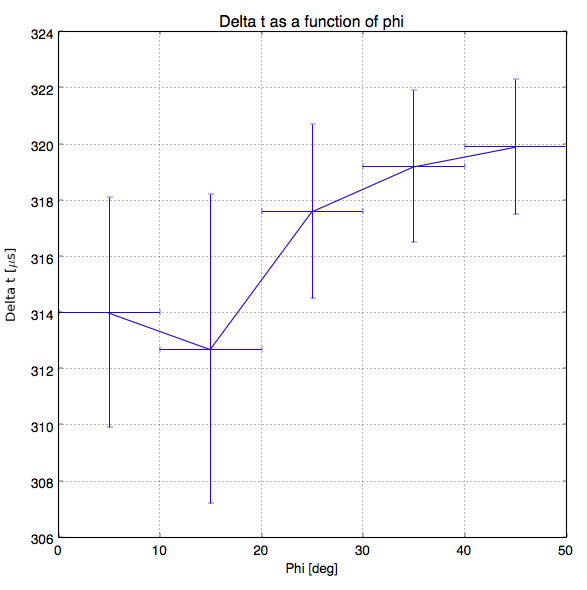
\includegraphics[width=3in]{images/CollectionFitRunIIPosPhi.png}
\caption{$\Delta$t for Run II positive polarity data  selected tracks as a function of Phi. }
\label{fig:RunIPosACPTheta}
\end{minipage}\hfill
\begin{minipage}{0.45\textwidth}
\centering
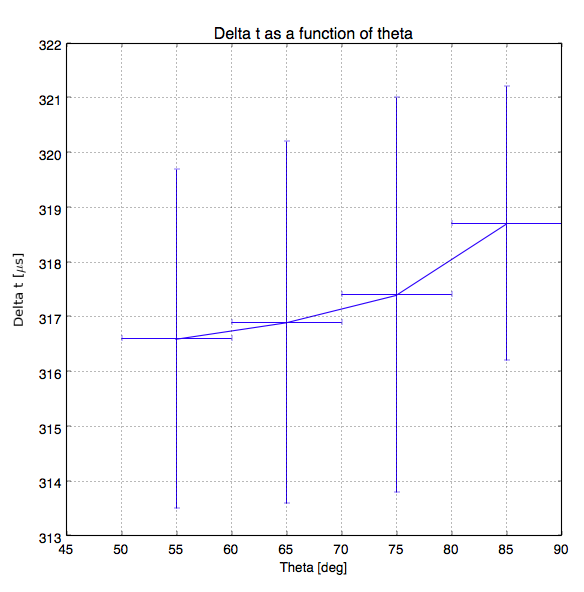
\includegraphics[width=3in]{images/CollectionFitRunIIPosTheta.png}
\caption{$\Delta$t for Run II positive polarity data ACP selected tracks as a function of Theta.}
\label{fig:RunIIPosACPPhi}
\end{minipage}
\end{figure}
\clearpage
\newpage
